\begin{figure}
	\centering
	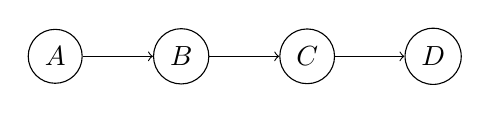
\begin{tikzpicture}[
		scale=0.8
	]

		\node[circle,draw=black] (A) at (-3,0) {$A$};
		\node[circle,draw=black] (B) at (-1,0) {$B$};
		\node[circle,draw=black] (C) at (1,0) {$C$};
		\node[circle,draw=black] (D) at (3,0) {$D$};

		\draw[->] (A) -- (B);
		\draw[->] (B) -- (C);
		\draw[->] (C) -- (D);

	\end{tikzpicture}
\end{figure}